\documentclass{standalone}
	\usepackage{tikz}
		\graphicspath{ {figures/AM_4_2/} }
	\begin{document}
\begin{tikzpicture}[node distance=0.01cm and 3cm]
 \node[anchor=center] (0) at (0,-0.8) { 4 \ (block2\_conv2) };
\node[anchor=center] at (6,-0.8) { 5 \ (block3\_conv1) };
 \foreach \label [count=\i] in {L3_F85.png,L3_F86.png,L3_F100.png,L3_F125.png,L3_F81.png} { 
 
	\node[draw=none] (\i) at (0,-\i*6em) {\includegraphics[width=0.3\textwidth]{\label} }; 
  }
\node[] (R) at (6,-3*6em) {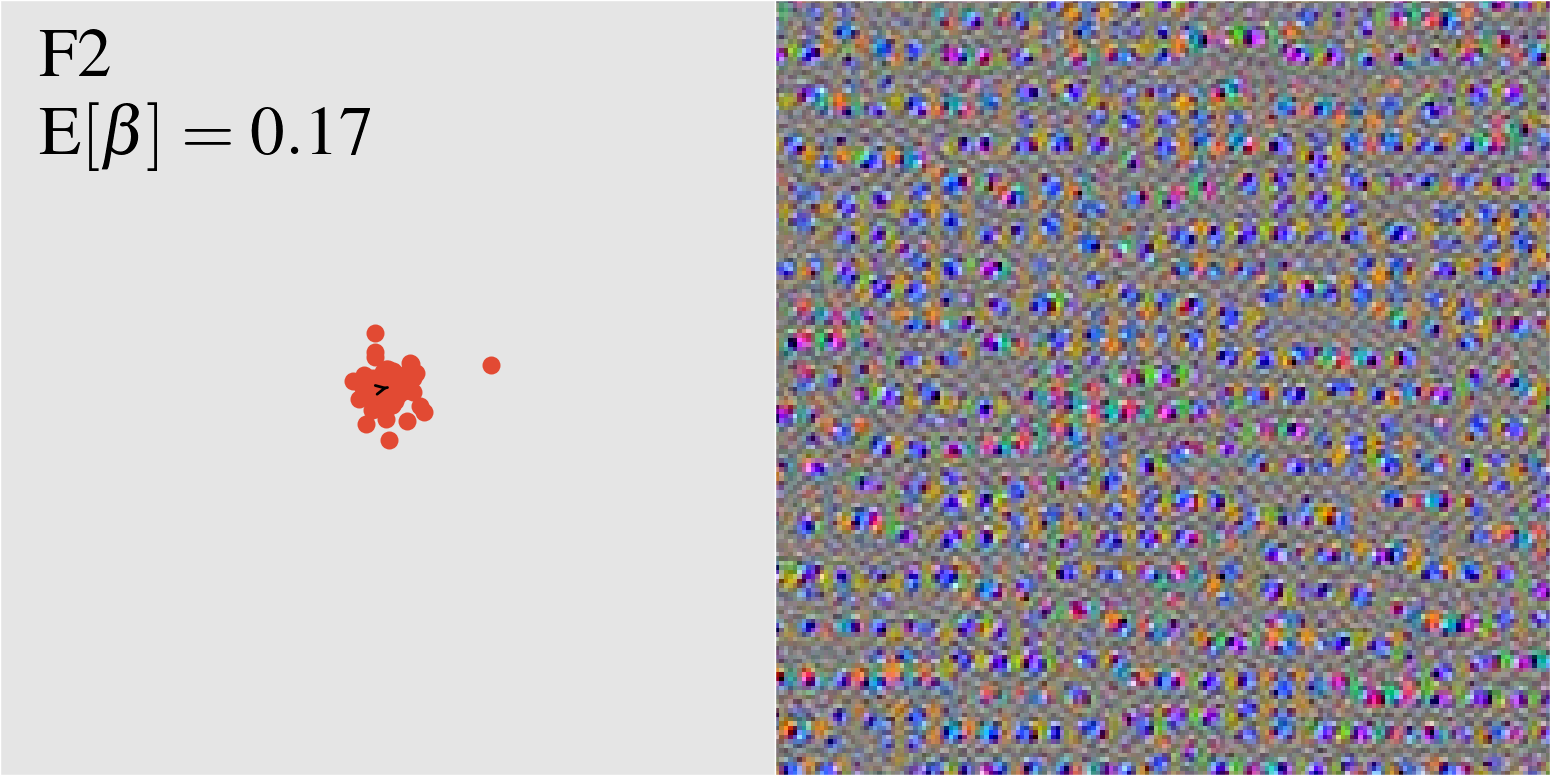
\includegraphics[width=0.3\textwidth]{ L4_F2.png } }; % Adjust the y-coordinate to center
 \draw (1.east) -- (R) node[pos=1, circle, draw, fill=white, minimum size=12pt, inner sep=0pt] {+}; 
 \draw (2.east) -- (R) node[pos=1, circle, draw, fill=white, minimum size=12pt, inner sep=0pt] {+}; 
 \draw (3.east) -- (R) node[pos=1, circle, draw, fill=white, minimum size=12pt, inner sep=0pt] {+}; 
 \draw (4.east) -- (R) node[pos=1, circle, draw, fill=white, minimum size=12pt, inner sep=0pt] {-}; 
 \draw (5.east) -- (R) node[pos=1, circle, draw, fill=white, minimum size=12pt, inner sep=0pt] {+}; 
\end{tikzpicture}
\end{document}
